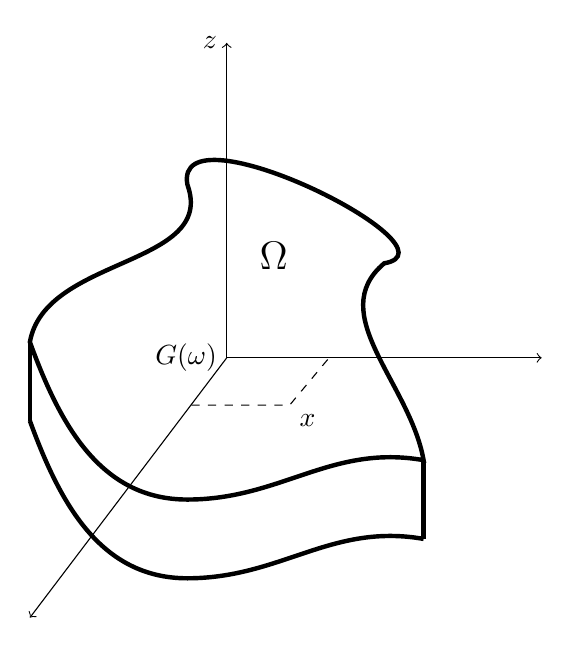
\begin{tikzpicture}
\node[coordinate] (v1) at (-3,3) {};
\node[coordinate] (v2) at (-5,1) {};
\node[coordinate] (v3) at (-3,-1) {};
\node[coordinate] (v4) at (0,-0.5) {};
\node[coordinate] (v5) at (-0.5,2) {};
%\draw  plot[smooth cycle, tension=.7] coordinates {(v5) (v1) (v2) (v3) (v4) (v5)};

\draw [ultra thick] (v1) to [out=290, in=80] (v2) to[out=290, in=180] (v3) to[out=0,in=170] (v4) to[out=100,in=220] (v5) to[out=10,in=100] (v1);

\node[coordinate] (v6) at (-5,0) {};
\node[coordinate] (v7) at (-3,-2) {};
\node[coordinate] (v8) at (0,-1.5) {};

\draw [ultra thick] (v2)--(v6); \draw [ultra thick] (v4)--(v8);
\draw [ultra thick]  (v6) to[out=290, in=180] (v7) to[out=0,in=170] (v8);

\node[coordinate] (v9) at (-2.5,0.8) {};
\node[coordinate] (v10) at (-5.0,-2.5) {};
\node[coordinate] (v11) at (1.5,0.8) {};
\node[coordinate] (v12) at (-2.5,4.8) {};

\draw [->] (v9)--(v10);
\draw [->] (v9)--(v11);
\draw [->] (v9)--(v12);


\node[left] (v9) at (-2.5,0.8) {$G(\omega)$};
\node[left] (v12) at (-2.5,4.8) {$z$};
\node[above left] (v13) at (-1.6,1.8) {\Large $\Omega$};

\node[coordinate] (v14) at (-1.2,0.8) {};
\node[coordinate] (v15) at (-1.7,0.2) {};
\node[coordinate] (v16) at (-2.95,0.2) {};
\draw[dashed] (v16)--(v15)--(v14);

\node[below right] (v15) at (-1.7,0.2) {$x$};

\end{tikzpicture}